\documentclass[a4paper]{article}
\usepackage{graphicx}
\graphicspath{/home/angelo/Documents/Uni/Courses/Advanced Statistics and programming/Assignments/assignment2/} 
\usepackage{mathtools}
\usepackage[a4paper, total={5in, 6.5in}]{geometry}
\usepackage{color}
\usepackage{tikz}
\usepackage{lipsum}
\usepackage{geometry}
\geometry{a4paper, left=2.5cm, top=2.5cm, bottom=2.5cm, right=2.5cm}
\usepackage{changepage}
\usepackage{booktabs}
\usepackage[font=small]{caption}
\DeclareCaptionFormat{mycaptionfont}{\fontsize{12}{13}\selectfont#1#2#3}
\usepackage{threeparttable}
\usepackage{ntheorem}
\usepackage{caption}
\usepackage{wrapfig,lipsum,booktabs}
\usepackage{listings}
\usepackage{pdflscape}
\captionsetup{format=mycaptionfont}
\usepackage{subcaption}
\theoremseparator{:}
\usepackage{lscape}

\usepackage[utf8]{inputenc}
\newtheorem{hyp}{Hypothesis}
\usetikzlibrary{shapes,decorations,arrows,calc,arrows.meta,fit,positioning}
\tikzset{
    -Latex,auto,node distance =1 cm and 1 cm,semithick,
    state/.style ={ellipse, draw, minimum width = 0.7 cm},
    point/.style = {circle, draw, inner sep=0.04cm,fill,node contents={}},
    bidirected/.style={Latex-Latex,dashed},
    el/.style = {inner sep=2pt, align=left, sloped}
}





\begin{document}

\title{ASAP Assignment 2}
\author{Angelo Barisano; 508903 }
\date{September 23rd, 2022}
\maketitle

\newpage
\section{Difference in Difference}


Description:
You are tasked with estimating the effects of the 1993 policy intervention on labor supply for single women by whether or not they had children.
--> The relevant varibales in this case are: 
state - US-State/ provice of residence
year - Year
urate - US-State/province unemployment rate
children - number of children per women
nonwhite - nonwhite
finc - annual family income
earn - anual earnings (of women)
age - age of women
ed - Years of education
work - Indicator work status (employed or not)
unearn - unearn Income 

Outcome variable: INDICATOR WORK STATUS
Time indicator: at 1993 (beginning) create time variable
Goal: estimate the effect of the 1993 policy intervention on labor supply for single women by whether or not they had children (Dummy for whether they had children or not??)


The unit of analysis are females in the US

Question: The main predictor is meant to be whether women has children; Should we use that as a dummy or numeric variable?? --> something like degree of treatment



\subsection{Indicate which of the coefficients(s) from equation (1) yield the following outcomes}

\textbf{NOte possibly delete duplicates}
SEE SLIDE 57 ff

Important: we canot identify the monthrs; so If they become mothers at some point, we will assume that these are taken out!



$
(1) {y_{it}} = \beta_{0} + \beta_{1} + \beta_{2} + \beta_{3} D_i T_t + \epsilon_{it}
$


$E = (y_{T=1} | D=1)$
$E = (y_{T=0} | D=1)$
$E = (y_{T=1} | D=0)$
$E = (y_{T=0} | D=0)$

$
[E(y_{T=1} | D=1) - E(y_{T=0} | D=1)] - [E(y_{T=1} | D=0) - E(y_{T=0} | D=0)]
$




\subsection{Task 2: Provide graphic as on slide 55}

\textbf{IMPORTANT: ALSO MENTION THE CATEGORICAL VARIABLES!!!}



\begin{wrapfigure}{L}{9cm}
\centering
\begin{subfigure}[b]{0.5\textwidth}
    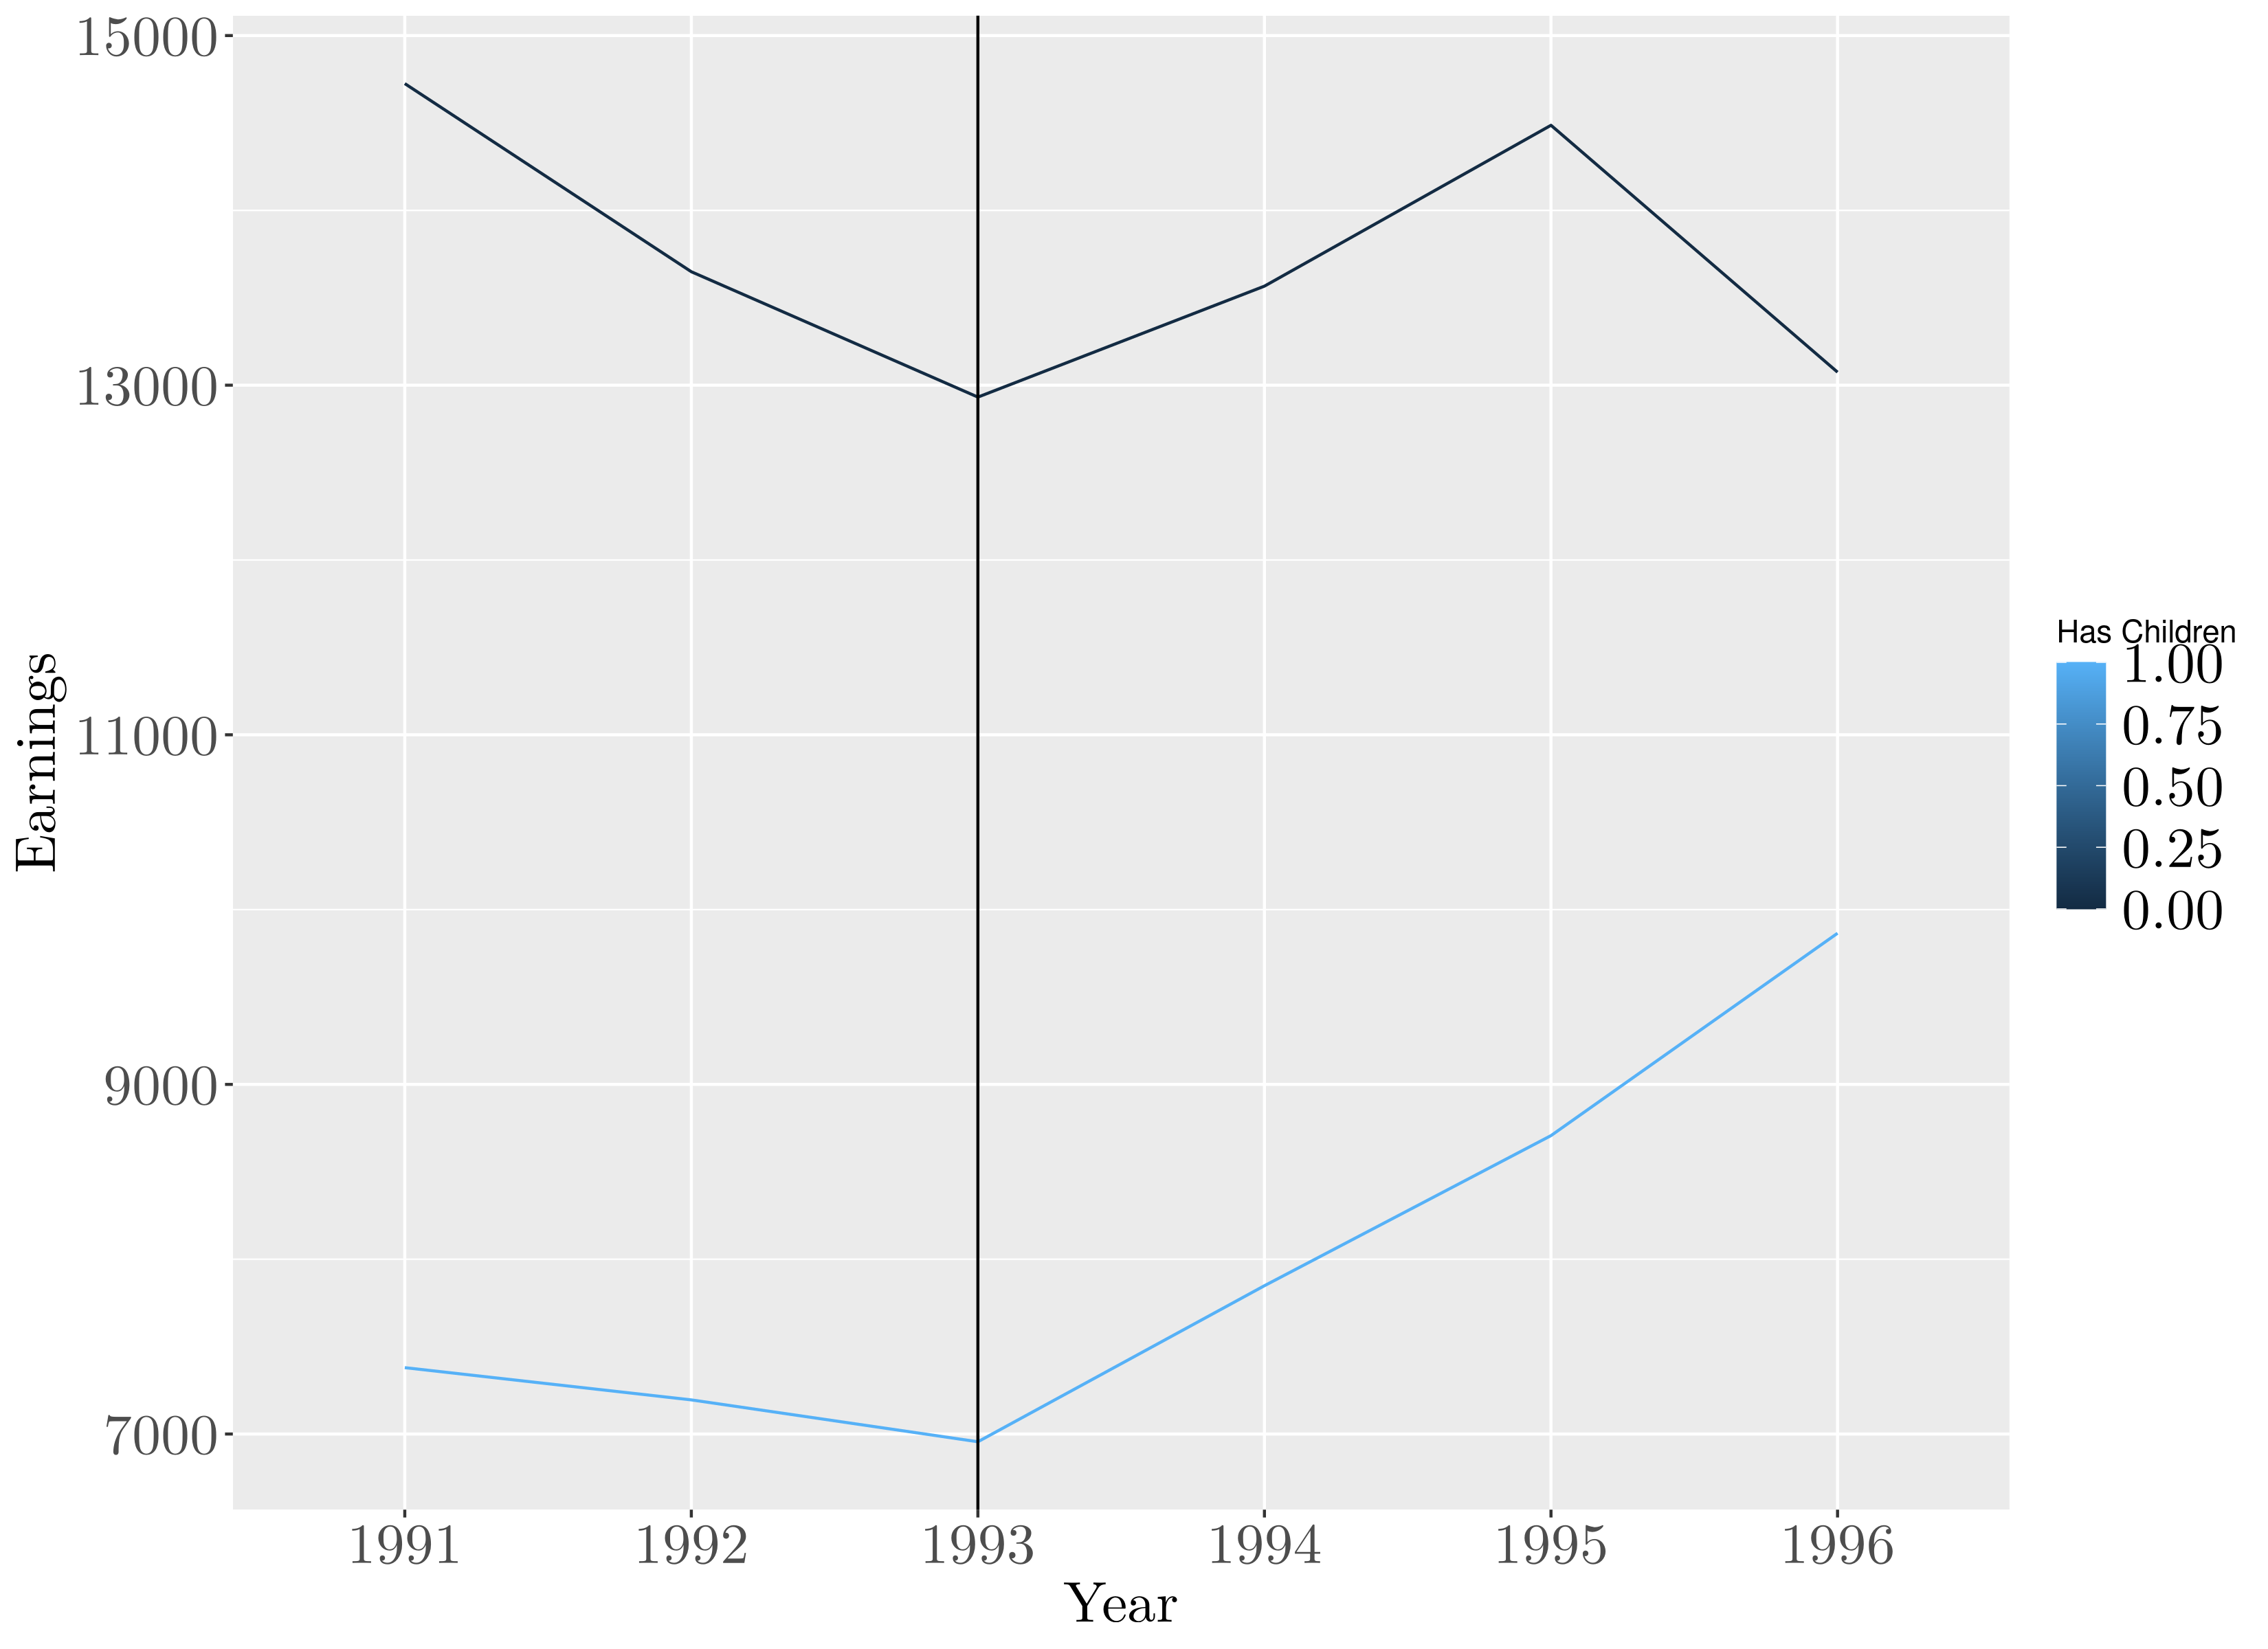
\includegraphics[width=.95\linewidth]{"/home/angelo/Documents/Uni/Courses/Advanced Statistics and programming/Assignments/assignment2/Graphics/task2_earn_did.png"} 
   \caption{Annual Earnings by Females with(out) Children}
   \label{fig:Ng2}
\end{subfigure}

\begin{subfigure}[b]{0.5\textwidth}
    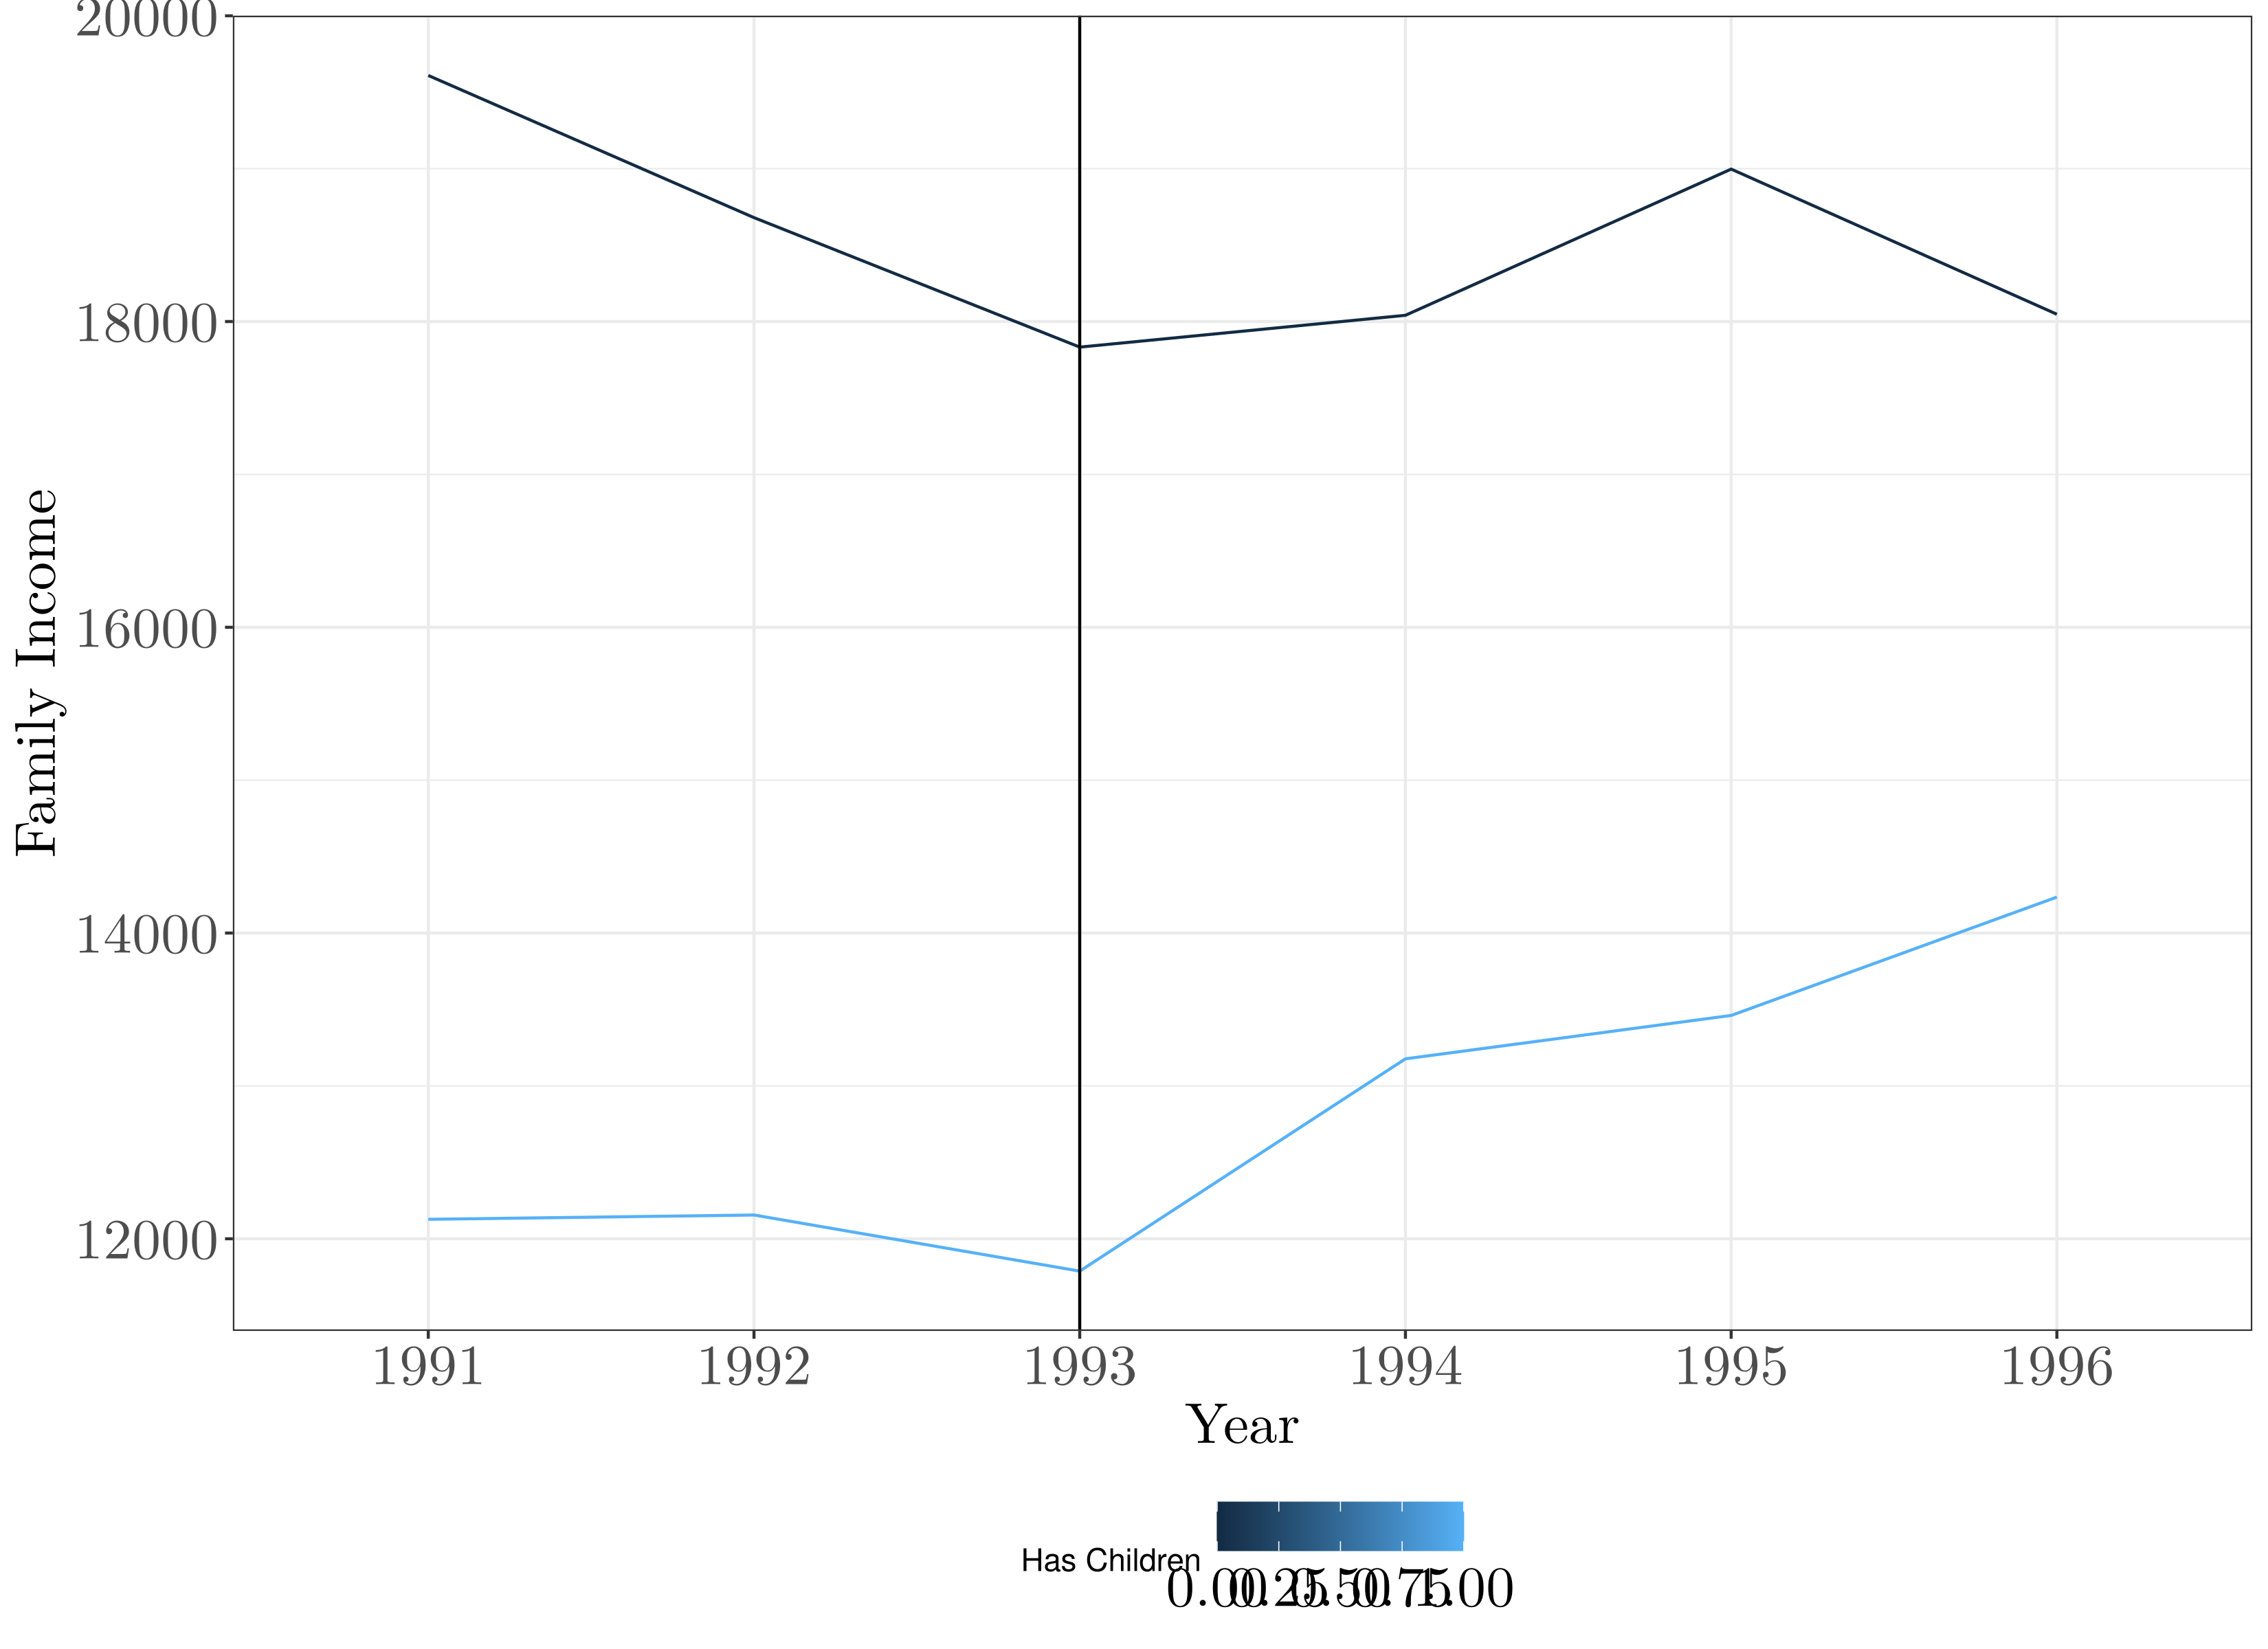
\includegraphics[width=.95\linewidth]{"/home/angelo/Documents/Uni/Courses/Advanced Statistics and programming/Assignments/assignment2/Graphics/task2_finc_did.png"} 
   \caption{Family Earnings Earnings by Females with(out) Children}
   \label{fig:Ng2}
\end{subfigure}

\begin{subfigure}[b]{0.5\textwidth}
    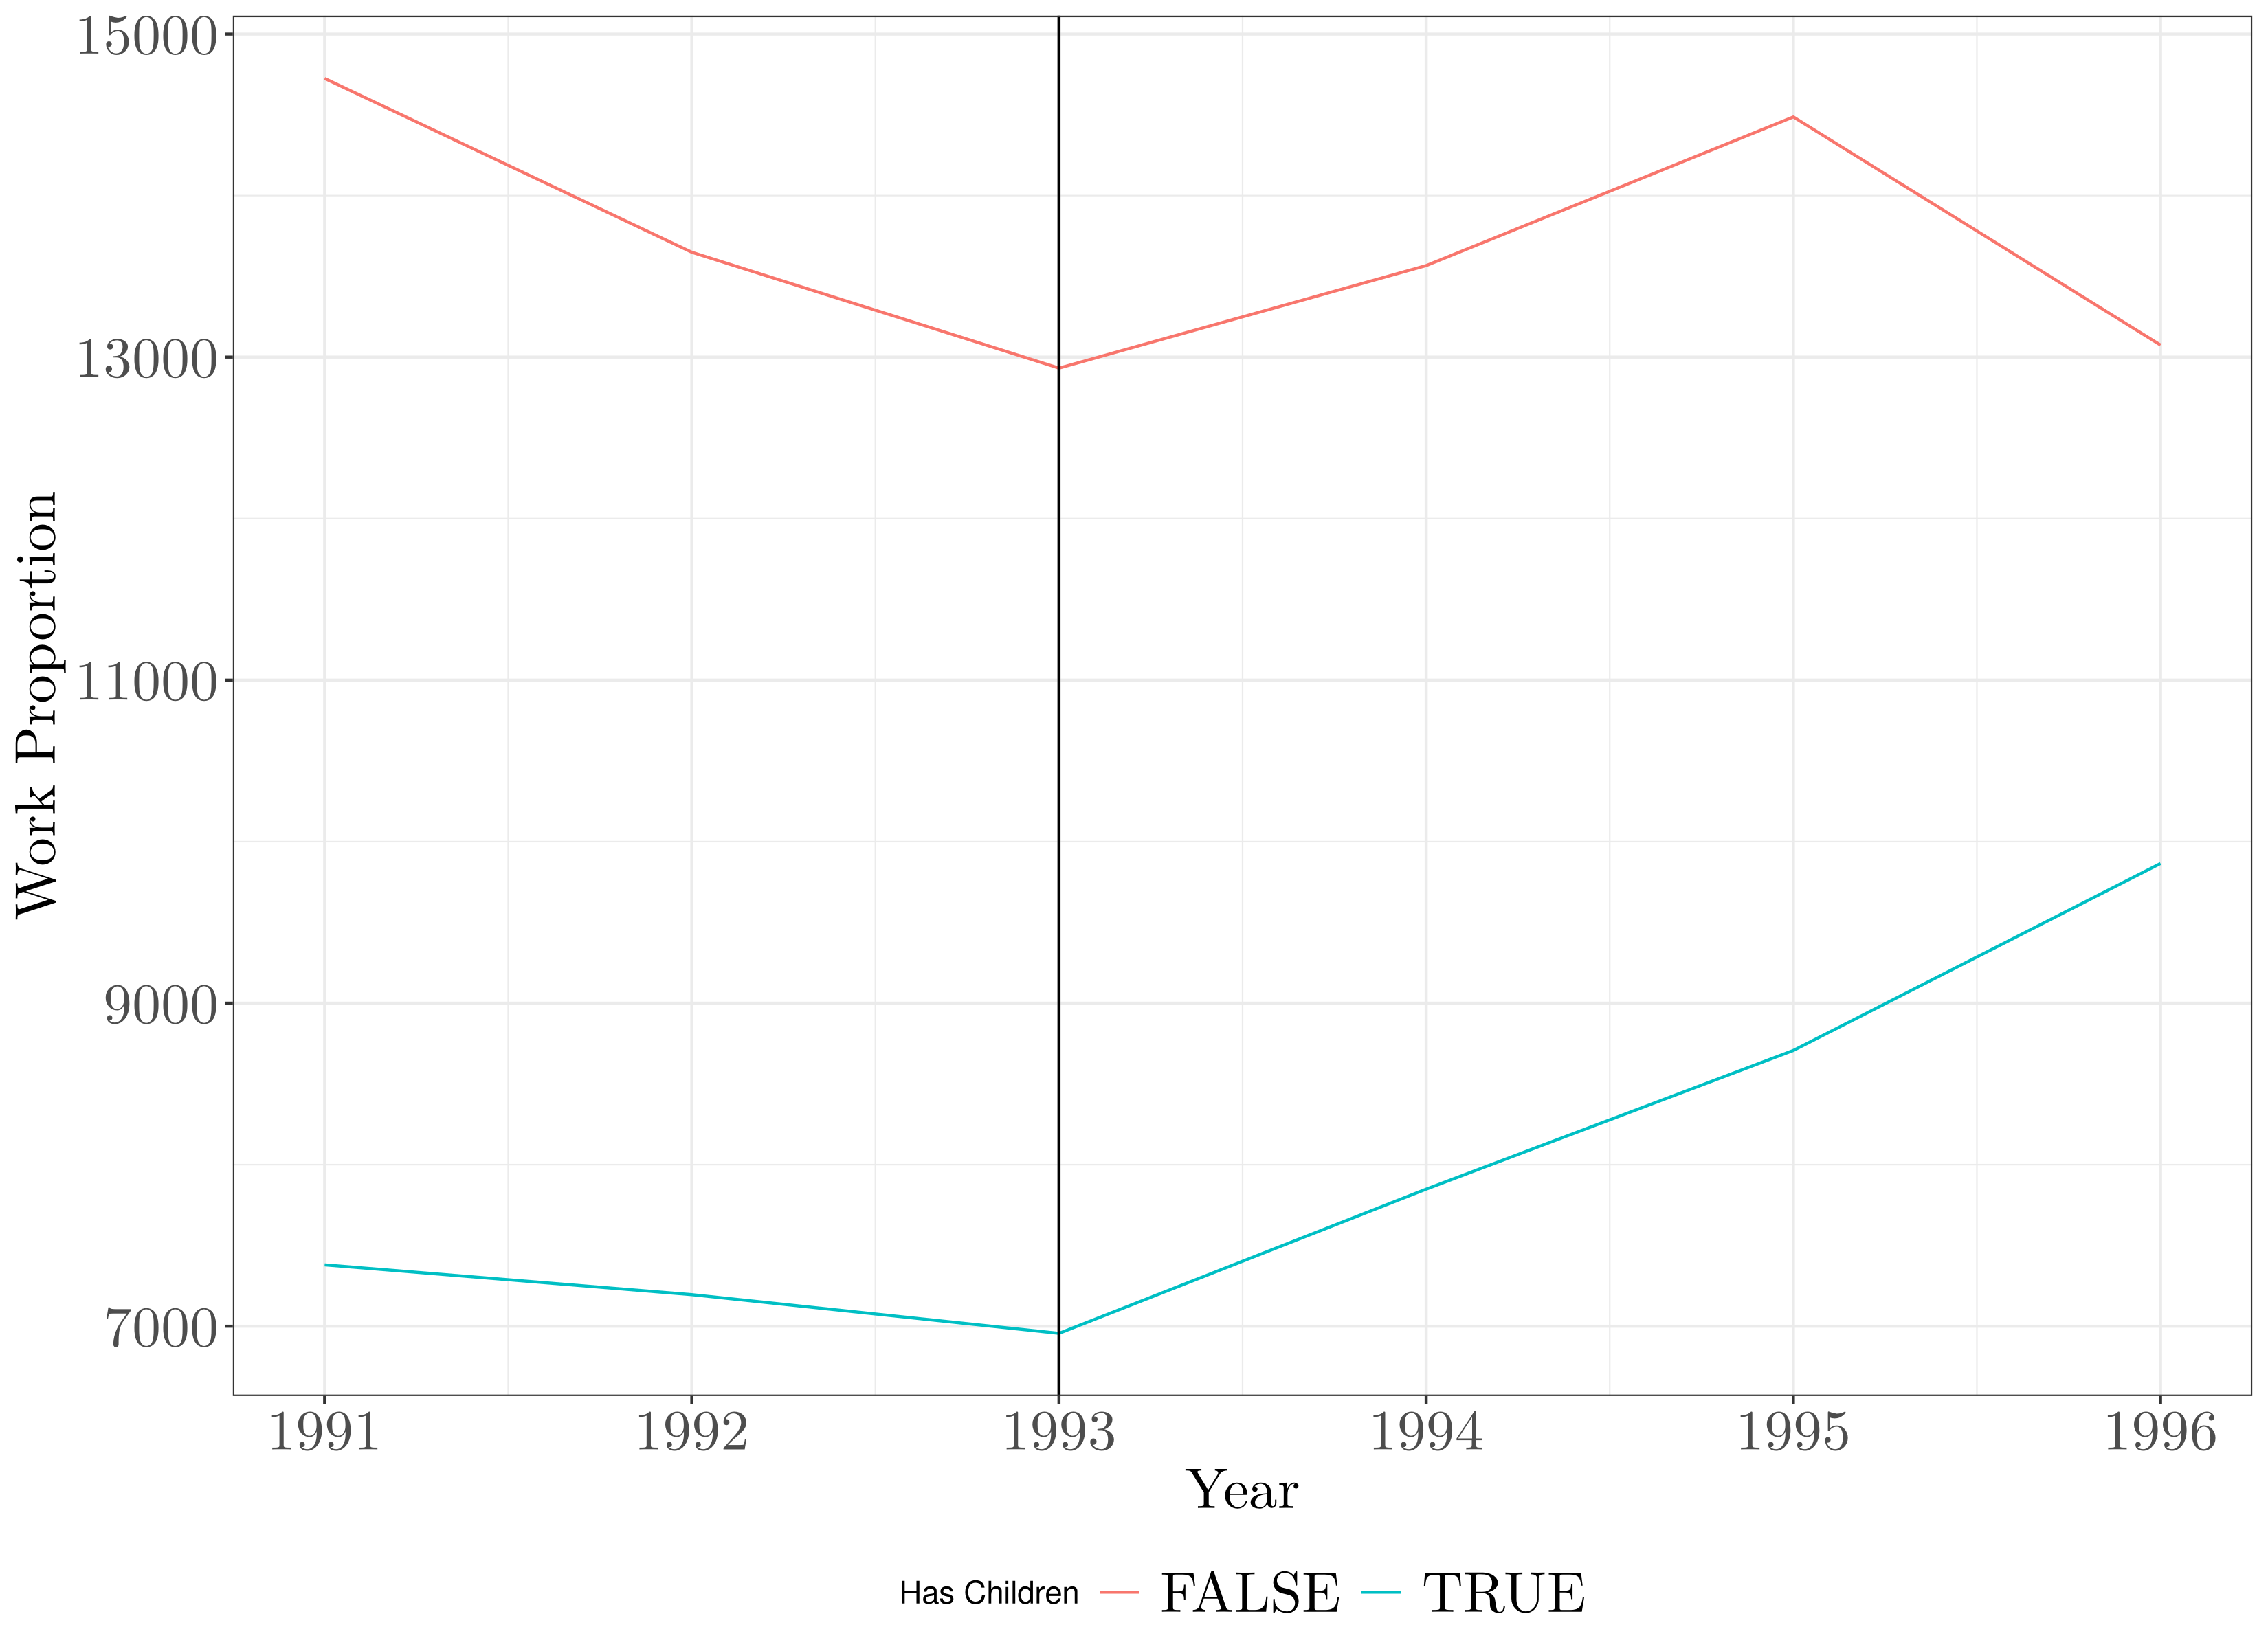
\includegraphics[width=.95\linewidth]{"/home/angelo/Documents/Uni/Courses/Advanced Statistics and programming/Assignments/assignment2/Graphics/task2_work_did.png"}  
   \caption{Work Participation by Females with(out) Children}
   \label{fig:Ng2}
\end{subfigure}
\captionsetup{justification=centering}
\caption{Pre-Post Intervention of EICT Credit for Women with(out) Children}
\end{wrapfigure}





NOTES: This "visoual" proof is no real proove; this is just visual confirmation of what we assume; but does this really pertain to the case that the TAX credit is the real cause? What about the case of subsections of the population? and we still do not know whether this is really causal and not like the economy heating up!`
Predictor is WHETHER YOU HAVE CHILD OR NOT


\subsection{Task 3: Summary Statistics for data}

% Table created by stargazer v.5.2.3 by Marek Hlavac, Social Policy Institute. E-mail: marek.hlavac at gmail.com
% Date and time: Fri, Sep 23, 2022 - 20:25:57
\begin{table}[!htbp] 
\begin{adjustwidth}{-0cm}{-0cm}
\begin{threeparttable}
\small
\captionsetup{font=small, justification=raggedright,singlelinecheck=false}
  \caption{Descriptive Statistics of Numeric Indepdenent and Dependent Varaible} 
  \label{} 
\begin{tabular}{@{\extracolsep{5pt}}lccccccc} 
\\[-1.8ex]\hline 
\hline \\[-1.8ex] 
Statistic & \multicolumn{1}{c}{Mean} & \multicolumn{1}{c}{St. Dev.} & \multicolumn{1}{c}{Min} & \multicolumn{1}{c}{Pctl(25)} & \multicolumn{1}{c}{Median} & \multicolumn{1}{c}{Pctl(75)} & \multicolumn{1}{c}{Max} \\ 
\hline \\[-1.8ex] 
Family Income & 15,255.320 & 19,444.250 & 0.000 & 5,123.418 & 9,636.664 & 18,659.180 & 575,616.800 \\ 
Earnings & 10,432.480 & 18,200.760 & 0.000 & 0.000 & 3,332.180 & 14,321.220 & 537,880.600 \\ 
Age & 35.210 & 10.157 & 20 & 26 & 34 & 44 & 54 \\ 
Education & 8.806 & 2.636 & 0 & 7 & 10 & 11 & 11 \\ 
Education Years & 4.823 & 7.123 & 0.000 & 0.000 & 2.973 & 6.864 & 134.058 \\ 
Unearned Income & 1.193 & 1.382 & 0 & 0 & 1 & 2 & 9 \\ 
Count Children & 0.513 & 0.500 & 0 & 0 & 1 & 1 & 1 \\ 
\hline \\[-1.8ex] 
\end{tabular} 
\begin{tablenotes}[para,flushleft]
      \small
      \item\textit{Notes:} N = 13746
    \end{tablenotes}
\end{threeparttable}
\end{adjustwidth}
\end{table}


% Table created by stargazer v.5.2.3 by Marek Hlavac, Social Policy Institute. E-mail: marek.hlavac at gmail.com
% Date and time: Fri, Sep 23, 2022 - 20:47:48
\begin{table}[!htbp] 
\begin{adjustwidth}{-0cm}{-0cm}
\begin{threeparttable}
\small
\captionsetup{font=small, justification=raggedright,singlelinecheck=false}
  \caption{Descriptive Statistics of ECIC; With Children} 
  \label{} 
\begin{tabular}{@{\extracolsep{5pt}}lccccccc} 
\\[-1.8ex]\hline 
\hline \\[-1.8ex] 
Statistic & \multicolumn{1}{c}{Mean} & \multicolumn{1}{c}{St. Dev.} & \multicolumn{1}{c}{Min} & \multicolumn{1}{c}{Pctl(25)} & \multicolumn{1}{c}{Median} & \multicolumn{1}{c}{Pctl(75)} & \multicolumn{1}{c}{Max} \\ 
\hline \\[-1.8ex] 
Family Income & 12,750.390 & 15,739.050 & 0.000 & 4,652.465 & 8,425.197 & 15,218.720 & 410,507.600 \\ 
Earnings & 7,909.934 & 14,956.930 & 0.000 & 0.000 & 1,110.727 & 11,107.270 & 366,095.500 \\ 
Age & 32.717 & 8.630 & 20 & 25 & 32 & 39 & 54 \\ 
Education & 9.001 & 2.408 & 0 & 7 & 10 & 11 & 11 \\ 
Education Years & 4.840 & 5.872 & 0.000 & 0.071 & 3.761 & 7.070 & 102.958 \\ 
Unearned Income & 2.097 & 1.209 & 1 & 1 & 2 & 3 & 9 \\ 
Count Children & 0.466 & 0.499 & 0 & 0 & 0 & 1 & 1 \\ 
\hline \\[-1.8ex] 
\end{tabular} 
\begin{tablenotes}[para,flushleft]
      \small
      \item\textit{Notes:} N = 7819
    \end{tablenotes}
\end{threeparttable}
\end{adjustwidth}
\end{table} 




% Table created by stargazer v.5.2.3 by Marek Hlavac, Social Policy Institute. E-mail: marek.hlavac at gmail.com
% Date and time: Fri, Sep 23, 2022 - 20:47:48
\begin{table}[!htbp] 
\begin{adjustwidth}{-0cm}{-0cm}
\begin{threeparttable}
\small
\captionsetup{font=small, justification=raggedright,singlelinecheck=false}
  \caption{Descriptive Statistics of ECIC; Without Children} 
  \label{} 
\begin{tabular}{@{\extracolsep{5pt}}lccccccc} 
\\[-1.8ex]\hline 
\hline \\[-1.8ex] 
Statistic & \multicolumn{1}{c}{Mean} & \multicolumn{1}{c}{St. Dev.} & \multicolumn{1}{c}{Min} & \multicolumn{1}{c}{Pctl(25)} & \multicolumn{1}{c}{Median} & \multicolumn{1}{c}{Pctl(75)} & \multicolumn{1}{c}{Max} \\ 
\hline \\[-1.8ex] 
Family Income & 18,559.860 & 23,041.780 & 0.000 & 5,793.092 & 11,912.950 & 24,391.010 & 575,616.800 \\ 
Earnings & 13,760.260 & 21,301.400 & 0.000 & 0.000 & 7,664.014 & 19,447.610 & 537,880.600 \\ 
Age & 38.498 & 11.046 & 20 & 28 & 40 & 49 & 54 \\ 
Education & 8.549 & 2.889 & 0 & 7 & 10 & 11 & 11 \\ 
Education Years & 4.800 & 8.496 & 0.000 & 0.000 & 1.248 & 6.528 & 134.058 \\ 
Unearned Income & 0.000 & 0.000 & 0 & 0 & 0 & 0 & 0 \\ 
Count Children & 0.574 & 0.494 & 0 & 0 & 1 & 1 & 1 \\ 
\hline \\[-1.8ex] 
\end{tabular} 
\begin{tablenotes}[para,flushleft]
      \small
      \item\textit{Notes:} N = 5927
    \end{tablenotes}
\end{threeparttable}
\end{adjustwidth}
\end{table}


\subsection{Task 4: Matrix Diff in Diff}
NOte: by taking the average of the periods we have two small problems: 1) the AFTER period is longer; so should we really do that?


% Table created by stargazer v.5.2.3 by Marek Hlavac, Social Policy Institute. E-mail: marek.hlavac at gmail.com
% Date and time: Fri, Sep 23, 2022 - 21:38:43
% Requires LaTeX packages: dcolumn 
\begin{table}[!htbp] 
\begin{adjustwidth}{-0cm}{-0cm}
\begin{threeparttable}
\small
\captionsetup{font=small, justification=raggedright,singlelinecheck=false}
  \caption{Diff-in-Diff Matrix} 
  \label{} 
\begin{tabular}{@{\extracolsep{8pt}}lccccccc} 
\\[-5.8ex]\hline 
\hline \\[-1.8ex]
\multicolumn{2}{c}{}  & \multicolumn{2}{c}{Earning}  & \multicolumn{2}{c}{Family Income} & \multicolumn{2}{c}{Work Participation} \\ 
\multicolumn{1}{c}{} & \multicolumn{1}{c}{dperiod} & \multicolumn{1}{c}{Childless} & \multicolumn{1}{c}{Has Child} & \multicolumn{1}{c}{Childless} & \multicolumn{1}{c}{Has Child} & \multicolumn{1}{c}{Childless} & \multicolumn{1}{c}{Has Child} \\ 
\hline \\[-1.8ex] 
\multicolumn{1}{c}{Before} & 1 & 14,203.900 & 7,290.380 & 19,159.190 & 12,140.900 & 0.580 & 0.450 \\ 
\multicolumn{1}{c}{After} & 2 & 13,507.900 & 8,277.200 & 18,218.950 & 13,111.690 & 0.570 & 0.480 \\ 
\multicolumn{1}{c}{Difference} &  & -696.000 & 986.810 & -940.240 & 970.800 & -0.010 & 0.030 \\ 
\hline \\[-3.6ex] 
\end{tabular} 
\begin{tablenotes}[para,flushleft]
      \small
      \item\textit{Notes:} N = 5927 Childless; N = 7819 Has one or more Children
    \end{tablenotes}
\end{threeparttable}
\end{adjustwidth}
\end{table}



\subsection{Task 5: Analyze the DiD effect with appropriate regression models for the three
dependent variables}
\textbf{NOTE STANDARDIZED COEFFICIENTS ARE NOT REPORTED AS THEY ARE USELESS IN THIS CONTEXT; WE ARE NOT LOOKIGN FOR EFFECT SIZE BUT RATHER THE CASE OF }


\textbf{Note:standardized coefficinets will NOT be included as they are of no interpretable interest here and there is no real effect size we want to estimate in the first place.}

\textbf{Also: give a short theroy for why control variables were included! LOOK AT PQRM QUANTITATIVE CORUSE AT UVA; THEY CALLED IT SOMETHING SPECIAL!}

\textbf{IMPORTANT: EXPLAIN WHY IN CERTAIN MODELS THE CONTROL VARIABLES WORK AND WHY THEY DONT WORK IN OTHER MODELS!! Build a theory in this regard }

\textbf{NOTE ROBUST STANDARD ERROS MIGHT NOT EVEN BE NEEDED IN THIS CASE DUE TO THE THEORY BEHIND DIFF IN DIFF }


\pagebreak

% Table created by stargazer v.5.2.3 by Marek Hlavac, Social Policy Institute. E-mail: marek.hlavac at gmail.com
% Date and time: Wed, Sep 14, 2022 - 15:53:27
\begin{table}[!htbp] \centering 
\begin{adjustwidth}{0.cm}{-0cm}
\begin{threeparttable}
\small
\captionsetup{font=small, justification=raggedright,singlelinecheck=false}
\caption{\textsc{Non-Robust Regression Results Part 3}}
\centering 
  \label{}
\small 
\begin{tabular}{@{\extracolsep{-2pt}}lcccccc} 
\\[-5.8ex]\hline 
\hline \\[-1.8ex] 
 & \multicolumn{6}{c}{\textit{Dependent variable:}} \\ 
\cline{2-7} 
\\[-1.8ex] & \multicolumn{2}{c}{earn} & \multicolumn{2}{c}{finc} & \multicolumn{2}{c}{work} \\ 
\\[-1.8ex] & (1) & (2) & (3) & (4) & (5) & (6)\\ 
\hline \\[-1.8ex] 
 Constant & 14,899.900$^{***}$ & 12,958.640$^{***}$ & 20,099.430$^{***}$ & 16,218.430$^{***}$ & 0.582$^{***}$ & 0.532$^{***}$ \\ 
  & (828.375) & (1,550.012) & (886.522) & (1,655.347) & (0.023) & (0.043) \\ 
  has\_children1 & $-$8,596.327$^{***}$ & $-$8,394.973$^{***}$ & $-$8,929.330$^{***}$ & $-$8,269.567$^{***}$ & $-$0.159$^{***}$ & $-$0.150$^{***}$ \\ 
  & (1,093.444) & (1,096.506) & (1,170.197) & (1,171.022) & (0.030) & (0.030) \\ 
  dperiod & $-$695.997 & $-$536.491 & $-$940.239$^{*}$ & $-$515.553 & $-$0.005 & $-$0.024$^{*}$ \\ 
  & (485.413) & (500.046) & (519.486) & (534.028) & (0.013) & (0.014) \\ 
  age &  & 22.555 &  & 78.717$^{***}$ &  & 0.002$^{***}$ \\ 
  &  & (15.922) &  & (17.004) &  & (0.0004) \\ 
  urate &  & 133.948 &  & 372.861$^{***}$ &  & $-$0.018$^{***}$ \\ 
  &  & (114.614) &  & (122.403) &  & (0.003) \\ 
  ed &  & 66.337 &  & $-$125.305$^{**}$ &  & 0.017$^{***}$ \\ 
  &  & (59.579) &  & (63.628) &  & (0.002) \\ 
  nonwhite1 &  & $-$1,255.622$^{***}$ &  & $-$2,438.387$^{***}$ &  & $-$0.043$^{***}$ \\ 
  &  & (326.237) &  & (348.408) &  & (0.009) \\ 
  has\_children1:dperiod & 1,682.810$^{***}$ & 1,722.360$^{***}$ & 1,911.035$^{***}$ & 2,006.060$^{***}$ & 0.031$^{*}$ & 0.033$^{*}$ \\ 
  & (642.099) & (641.893) & (687.171) & (685.515) & (0.018) & (0.018) \\ 
 \hline \\[-1.8ex] 
R$^{2}$ & 0.026 & 0.027 & 0.022 & 0.028 & 0.012 & 0.027 \\ 
Adjusted R$^{2}$ & 0.026 & 0.027 & 0.022 & 0.027 & 0.012 & 0.026 \\ 
Residual Std. Error & 17,965.670 & 17,956.450  & 19,226.750  & 19,176.730 & 0.497  & 0.493  \\ 
F Statistic & 121.691$^{***}$ & 54.794$^{***}$ & 105.245$^{***}$ & 56.166$^{***}$  & 54.906$^{***}$  & 54.374$^{***}$  \\ 
\hline 
\hline \\[-3.5ex] 
\end{tabular} 
\begin{tablenotes}[para,flushleft]
      \small
      \item\textit{Note:} N = 13746. Non Robust Standard Errors applied. "White" is reference category for "non-White" categorical variable.
    \end{tablenotes}
\end{threeparttable}
\end{adjustwidth}
%
\end{table}





\subsection{Task 6: Subset analysis}
\textbf{NOTE: IN THIS CASE WE USE THE SUBSET ANALYSIS and not use interactions due to the efficeincy; if we were to use interactions, the analysis would have a higher statistical power, but the problem is: it would be really difficult to discern }

\textbf{NOTE WE STILL USE DIFF IN DIFF BECAUSE WE STILL WANT TO SEE THE EFFECT OF THE POLICY INTERVATION JUST HERE SUBSECTIONED BY DIFFERENT VARIABLES }

\subsubsection{Women with Children compared based on high \& low education levels}
% Table created by stargazer v.5.2.3 by Marek Hlavac, Social Policy Institute. E-mail: marek.hlavac at gmail.com
% Date and time: Wed, Sep 14, 2022 - 15:53:27
\begin{table}[!htbp] \centering 
\begin{adjustwidth}{0.cm}{-0cm}
\begin{threeparttable}
\small
\captionsetup{font=small, justification=raggedright,singlelinecheck=false}
\caption{\textsc{Subsection Analysis Single Women with Children for alternating low/ high education levels}}
\centering 
  \label{}
\small 
\begin{tabular}{@{\extracolsep{-2pt}}lcccccc} 
\\[-5.8ex]\hline 
\hline \\[-1.8ex] 
 & \multicolumn{6}{c}{\textit{Dependent variable:}} \\ 
\cline{2-7} 
\\[-1.8ex] & \multicolumn{2}{c}{earn} & \multicolumn{2}{c}{finc} & \multicolumn{2}{c}{work} \\ 
\\[-1.8ex] & (1) & (2) & (3) & (4) & (5) & (6)\\ 
\hline \\[-1.8ex] 
 Constant & 14,899.900$^{***}$ & 12,958.640$^{***}$ & 20,099.430$^{***}$ & 16,218.430$^{***}$ & 0.582$^{***}$ & 0.532$^{***}$ \\ 
  & (828.375) & (1,550.012) & (886.522) & (1,655.347) & (0.023) & (0.043) \\ 
  has\_children1 & $-$8,596.327$^{***}$ & $-$8,394.973$^{***}$ & $-$8,929.330$^{***}$ & $-$8,269.567$^{***}$ & $-$0.159$^{***}$ & $-$0.150$^{***}$ \\ 
  & (1,093.444) & (1,096.506) & (1,170.197) & (1,171.022) & (0.030) & (0.030) \\ 
  dperiod & $-$695.997 & $-$536.491 & $-$940.239$^{*}$ & $-$515.553 & $-$0.005 & $-$0.024$^{*}$ \\ 
  & (485.413) & (500.046) & (519.486) & (534.028) & (0.013) & (0.014) \\ 
  age &  & 22.555 &  & 78.717$^{***}$ &  & 0.002$^{***}$ \\ 
  &  & (15.922) &  & (17.004) &  & (0.0004) \\ 
  urate &  & 133.948 &  & 372.861$^{***}$ &  & $-$0.018$^{***}$ \\ 
  &  & (114.614) &  & (122.403) &  & (0.003) \\ 
  ed &  & 66.337 &  & $-$125.305$^{**}$ &  & 0.017$^{***}$ \\ 
  &  & (59.579) &  & (63.628) &  & (0.002) \\ 
  nonwhite1 &  & $-$1,255.622$^{***}$ &  & $-$2,438.387$^{***}$ &  & $-$0.043$^{***}$ \\ 
  &  & (326.237) &  & (348.408) &  & (0.009) \\ 
  has\_children1:dperiod & 1,682.810$^{***}$ & 1,722.360$^{***}$ & 1,911.035$^{***}$ & 2,006.060$^{***}$ & 0.031$^{*}$ & 0.033$^{*}$ \\ 
  & (642.099) & (641.893) & (687.171) & (685.515) & (0.018) & (0.018) \\ 
 \hline \\[-1.8ex] 
Observations & 13,746 & 13,746 & 13,746 & 13,746 & 13,746 & 13,746 \\ 
R$^{2}$ & 0.026 & 0.027 & 0.022 & 0.028 & 0.012 & 0.027 \\ 
Adjusted R$^{2}$ & 0.026 & 0.027 & 0.022 & 0.027 & 0.012 & 0.026 \\ 
Residual Std. Error & 17,965.670 & 17,956.450  & 19,226.750  & 19,176.730 & 0.497 & 0.493 \\ 
F Statistic & 121.691$^{***}$ & 54.794$^{***}$ & 105.245$^{***}$ & 56.166$^{***}$ & 54.906$^{***}$ & 54.374$^{***}$  \\ 
\hline 
\hline \\[-3.5ex] 
\end{tabular} 
\begin{tablenotes}[para,flushleft]
      \small
      \item\textit{Note:} N = 7819 Single Women have Children. N = 5593 high education (years of eduction $>$= 9 years); N = 2226 low education (years of eduction $<$ 9 years); Non Robust Standard Errors applied. "White" is reference category for "non-White" categorical variable.
    \end{tablenotes}
\end{threeparttable}
\end{adjustwidth}
%
\end{table}

\subsubsection{Women with and without Children compared keeping education level (low) constant}

% Table created by stargazer v.5.2.3 by Marek Hlavac, Social Policy Institute. E-mail: marek.hlavac at gmail.com
% Date and time: Wed, Sep 14, 2022 - 15:53:27
\begin{table}[!htbp] \centering 
\begin{adjustwidth}{0.cm}{-0cm}
\begin{threeparttable}
\small
\captionsetup{font=small, justification=raggedright,singlelinecheck=false}
\caption{\textsc{Subsection Analysis Single Women with/ without Children for constant (low) education levels}}
\centering 
  \label{}
\small 
\begin{tabular}{@{\extracolsep{-2pt}}lcccccc} 
\\[-5.8ex]\hline 
\hline \\[-1.8ex] 
 & \multicolumn{6}{c}{\textit{Dependent variable:}} \\ 
\cline{2-7} 
\\[-1.8ex] & \multicolumn{2}{c}{earn} & \multicolumn{2}{c}{finc} & \multicolumn{2}{c}{work} \\ 
\\[-1.8ex] & (1) & (2) & (3) & (4) & (5) & (6)\\ 
\hline \\[-1.8ex] 
 Constant & 11,066.700$^{***}$ & 4,281.758 & 17,494.530$^{***}$ & 8,507.214$^{***}$ & 0.501$^{***}$ & 0.441$^{***}$ \\ 
  & (1,457.343) & (2,602.848) & (1,534.185) & (2,735.084) & (0.038) & (0.068) \\ 
  has\_children1 & $-$2,323.038 & $-$2,402.722 & $-$3,739.399$^{*}$ & $-$3,267.950 & $-$0.080 & $-$0.087 \\ 
  & (2,026.514) & (2,030.169) & (2,133.367) & (2,133.311) & (0.053) & (0.053) \\ 
  dperiod & 783.677 & 1,378.102 & 322.393 & 1,127.629 & $-$0.004 & $-$0.007 \\ 
  & (858.662) & (882.127) & (903.937) & (926.943) & (0.023) & (0.023) \\ 
  age &  & 29.868 &  & 83.479$^{***}$ &  & 0.001 \\ 
  &  & (29.856) &  & (31.373) &  & (0.001) \\ 
  urate &  & 651.163$^{***}$ &  & 845.832$^{***}$ &  & $-$0.002 \\ 
  &  & (216.731) &  & (227.742) &  & (0.006) \\ 
  nonwhite1 &  & 332.812 &  & $-$2,403.220$^{***}$ &  & 0.081$^{***}$ \\ 
  &  & (664.392) &  & (698.146) &  & (0.017) \\ 
  has\_children1:dperiod & $-$413.449 & $-$475.403 & $-$179.637 & $-$152.761 & 0.015 & 0.012 \\ 
  & (1,194.473) & (1,193.612) & (1,257.455) & (1,254.253) & (0.031) & (0.031) \\ 
 \hline \\[-1.8ex] 
Observations & 4,311 & 4,311 & 4,311 & 4,311 & 4,311 & 4,311 \\ 
R$^{2}$ & 0.006 & 0.009 & 0.010 & 0.016 & 0.003 & 0.008 \\ 
Adjusted R$^{2}$ & 0.006 & 0.008 & 0.009 & 0.015 & 0.002 & 0.007 \\ 
Residual Std. Error & 18,962.540 & 18,944.100  & 19,962.390  & 19,906.540 & 0.498 & 0.497  \\ 
F Statistic & 9.304$^{***}$  & 6.559$^{***}$ & 14.690$^{***}$  & 11.920$^{***}$ & 4.494$^{***}$  & 6.121$^{***}$  \\ 
\hline 
\hline \\[-3.5ex] 
\end{tabular} 
\begin{tablenotes}[para,flushleft]
      \small
      \item\textit{Note:} N = 4411 Single Women have Children (years of eduction $<$ 9 years). N = 2085 has no children; N = 2226 has children; Non Robust Standard Errors applied. "White" is reference category for "non-White" categorical variable.
    \end{tablenotes}
\end{threeparttable}
\end{adjustwidth}
%
\end{table}




\pagebreak

\section{Tart 2 Instrumental Variable approach}


Notes:
- Effect of cumpulsory schooling on wages

Generaly: the quality and quantitiy of education in modern societies is on a steady rise; but it is difficult how much education contributes to future earnings on the labor market.. meansing: how much does one year of additional education add in earnings

This is because of unobserved factors that are to the detrimetn of assumtion 3 (mean independence) biasing any OLS estimate of wages on years of eduction (ommitted variables and confounders).

Here the solution: instruments to circumvent these biases; combining to characteristics: 
--> Minimum legal school dropout age (which can be 16, 17, or 18 years) 
--> and the annual quarter of birth of a person

Rational behind these choices: all students born in the sam year are admitted to school in the same cohort (the same class). BUT A student born in eg January reaches the leagal school dropout age earlier than a student born in September 8eg).

--> as such, the instruments function as if; we randomize school exposure to students, assuming that in each year, a constant fraction of students drops out of school adn this dorpout pattern is unrelated to when a students is born. 

\textbf{MAIN TASK: Estimate the effect of the yerars of education on the LOG scaled wages}

\subsection{Explain wHY ols is biased here - A3}
--> IMPORTANT: ALSO INCLDUE 1) THE METHOD OF IV being different than least squares (it is a method look up in notes) and 2) mention the two requirements for a good Instrument: a) cleanliness no impact on outcome causally only through the biased independent varaible and b) the relevance which is high correlcion with the independent varaibvles that are instrumentalized

\textbf{In this exercies give two examples of conditions that could bias the estimated education effect if only OLS is used; This means: give examples how the variable YEARSOFEDUCATION is a biased estimator becasue mean independece is violated --> the example given was: students preference for education may influence how long they stay in school and how much they earn on the labor market which is simply their ambition; other factors might be: family background and societal status/ socioeconomic status which means something like teen pregnancy OR IN THE 1930s during the great depression just the need to support the family during time of need so you could not go to school}


\subsection{Summary statistics for this task}

relevant quantiative variables age, educ (years of education), lnwage(weekly earnings), marrital status; quarter of birth of the recorded child; SMSA: categorical variable where someone lives (urban vs not urban); yob year of birth which is also categorical

--> possibly retransform lnwage to just wage by reversing the log scaling


% Table created by stargazer v.5.2.3 by Marek Hlavac, Social Policy Institute. E-mail: marek.hlavac at gmail.com
% Date and time: Sun, Sep 25, 2022 - 15:43:50
\begin{table}[!htbp] 
\begin{adjustwidth}{-0cm}{-0cm}
\begin{threeparttable}
\small
\captionsetup{font=small, justification=raggedright,singlelinecheck=false}
  \caption{Instrumental Vairable Approach Descriptive Statistics of Numeric Indepdenent and Dependent Varaible} 
  \label{} 
\begin{tabular}{@{\extracolsep{5pt}}lccccccc} 
\\[-1.8ex]\hline 
\hline \\[-1.8ex] 
Statistic & \multicolumn{1}{c}{Mean} & \multicolumn{1}{c}{St. Dev.} & \multicolumn{1}{c}{Min} & \multicolumn{1}{c}{Pctl(25)} & \multicolumn{1}{c}{Median} & \multicolumn{1}{c}{Pctl(75)} & \multicolumn{1}{c}{Max} \\ 
\hline \\[-1.8ex] 
Age & 44.645 & 2.940 & 40 & 42 & 45 & 47 & 50 \\ 
Years of Education & 12.770 & 3.281 & 0 & 12 & 12 & 15 & 20 \\ 
Ln(Wage) & 5.900 & 0.679 & $-$2.342 & 5.637 & 5.952 & 6.257 & 10.532 \\ 
\hline \\[-3.5ex] 
\end{tabular} 
\begin{tablenotes}[para,flushleft]
      \small
      \item\textit{Notes:} N = 13746; Wage is backwards transformed from lnWage
    \end{tablenotes}
\end{threeparttable}
\end{adjustwidth}
\end{table}


\end{document}
